%% ============================================================
%% Section 1: Introduction (V0.2)
%% Target: ~1,300 words
%% Changes from V0.1: AIGC definition expanded (+ action),
%%   §4/§5 swapped in organization, Arup compressed,
%%   contribution 4 reframed, Figure 1 updated
%% ============================================================

\section{Introduction}
\label{sec:introduction}

%% --- P1: The Rise of AIGC + expanded definition (~350 words) ---

The release of ChatGPT in November 2022 marked the beginning of a generative AI revolution that has fundamentally transformed the digital landscape. In under three years, generative models have advanced from producing passable but detectable text to generating photorealistic images, pixel-perfect video, and voice clones indistinguishable from reality---all at near-zero marginal cost. We define \emph{AI-Generated Content} (AIGC) broadly as any artifact---text, images, audio, video, code, \emph{or action}---produced by generative artificial intelligence systems. The inclusion of \emph{action} reflects a critical architectural shift: vision-language-action (VLA) models and LLM-based agents tokenize real-world operations (tool calls, API requests, shell commands) as generated sequences structurally identical to language tokens~\cite{wang2024agentsurvey}. When the boundary of AIGC extends from static content to autonomous action, the security threat paradigm escalates correspondingly---from ``AI produces harmful content'' to ``AI autonomously executes harmful operations in real computing environments.''

Capability milestones across modalities underscore the scale of this transformation. Frontier LLMs---GPT-4~\cite{gpt4}, Claude, Gemini~\cite{gemini2024}, Llama~\cite{llama3}, and DeepSeek-V3~\cite{deepseekv3}---match or exceed human performance on professional writing and graduate-level reasoning. In image synthesis, human observers correctly identify AI-generated images only 53--61\% of the time~\cite{microsoft2025human}. Neural codec models such as VALL-E~\cite{wang2023valle} enable voice cloning from three seconds of audio. Video generators including Sora~\cite{brooks2024sora} and Veo~2 produce temporally consistent, high-resolution output. The adoption scale is commensurate: ChatGPT reached 100~million users within two months, the generative AI market is projected to exceed \$200~billion by 2030, and a rapidly growing fraction of internet content is now AI-generated~\cite{graphite2025aicontent}.

%% --- P2: The Urgency of Security and Safety Challenges (~300 words) ---

This transformative capability carries a dual nature. While AIGC delivers unprecedented benefits across education, healthcare, and software engineering, it simultaneously introduces severe \emph{security} and \emph{safety} challenges.

On the \textbf{security} dimension, generative AI has created novel attack vectors: adversarial manipulation via prompt injection and jailbreaking, data poisoning and backdoor attacks on training pipelines, supply chain vulnerabilities in open-weight model ecosystems, and---most critically---agentic exploitation, where autonomous AI agents execute multi-step attacks in real computing environments (Section~\ref{sec:cap-autonomy}). On the \textbf{safety} dimension, AIGC enables industrial-scale deepfake production (Section~\ref{sec:threat-deepfake}), hyper-personalized disinformation (Section~\ref{sec:threat-infoop}), non-consensual intimate imagery (Section~\ref{sec:threat-ncii}), bias amplification (Section~\ref{sec:threat-bias}), and privacy leakage through training data memorization.

The urgency is grounded in operational reality. The Arup deepfake fraud (\$25M, January 2024) demonstrated video-conference impersonation at catastrophic scale~\cite{brightside2025phishing}. An estimated 82.6\% of phishing emails in 2025 were AI-generated~\cite{knowbe4_2025}. The 2024 ``super election year'' saw documented AI interference across Taiwan, Indonesia, India, and the EU~\cite{restofworld2024tracker}. The international community has responded: the AI Safety Summit series (Bletchley Park $\to$ Seoul $\to$ Paris $\to$ New Delhi), the International AI Safety Reports~\cite{aisafetyreport2025,aisafetyreport2026}, and the EU AI Act~\cite{euaiact2024} all reflect recognition that AIGC risks have crossed from hypothetical concern to operational crisis.

%% --- P3: Contributions and Positioning (~350 words) ---

Existing surveys address fragments of this landscape: deepfake detection~\cite{pei2024deepfakesurvey}, AI-enabled influence operations~\cite{spitale2023gpt3}, LLM vulnerability catalogs~\cite{owasp2025}, and international safety assessments~\cite{aisafetyreport2025,aisafetyreport2026}. However, none systematically covers the full spectrum from content-generation risks through autonomous agentic exploitation, nor bridges technical analysis with governance and ethical perspectives.

This survey makes four contributions:
\begin{enumerate}[nosep,leftmargin=1.5em]
    \item \textbf{Security + Safety dual-dimensional threat taxonomy.} We propose a structured taxonomy (Section~\ref{sec:threats}) distinguishing security threats (adversarial compromise of AI systems) from safety threats (harmful outputs and societal impacts), covering content weaponization, model-level attacks, adversarial manipulation, misinformation, and ethical risks.
    \item \textbf{Attack surface evolution ladder as an original analytical framework.} We trace the escalation from direct prompt injection through jailbreaking and indirect prompt injection to agentic exploitation via the Model Context Protocol (MCP) ecosystem---to our knowledge, the first AIGC survey to systematically map this progression (Sections~\ref{sec:cap-autonomy} and~\ref{sec:threat-adversarial}).
    \item \textbf{Cross-disciplinary analysis spanning technology, policy, and ethics.} We bridge technical countermeasures (Section~\ref{sec:countermeasures}) with governance frameworks across the EU, US, and China (Section~\ref{sec:governance}), and ethical considerations including bias, copyright, and accountability (Section~\ref{sec:threat-ethics}).
    \item \textbf{Emphasis on agentic exploitation as the emerging frontier.} Beyond full-modality coverage incorporating 2025--2026 developments, this survey foregrounds the qualitative shift from content risks to action risks---where AI agents with tool-invocation privileges represent the most consequential and least-governed threat vector.
\end{enumerate}

%% --- P4: Paper Organization (~200 words) ---

The remainder of this paper is organized as follows. Section~\ref{sec:capabilities} examines the generative AI capabilities that make current challenges unprecedentedly severe, organized by four threat-relevant properties: high-fidelity generation, low-cost production, controllability, and autonomous agency. Section~\ref{sec:threats} presents the core threat taxonomy, including the novel attack surface evolution ladder from prompt injection to agentic exploitation. Section~\ref{sec:countermeasures} surveys technical countermeasures spanning detection, watermarking, alignment, adversarial defense, and agentic security. Section~\ref{sec:governance} analyzes the governance landscape, comparing regulatory frameworks and industry self-regulation. Section~\ref{sec:future} identifies six open research frontiers. Section~\ref{sec:conclusions} concludes with a synthesis of key insights. Figure~\ref{fig:structure} illustrates the paper's structure and logical dependencies.

\begin{figure}[htbp]
\centering
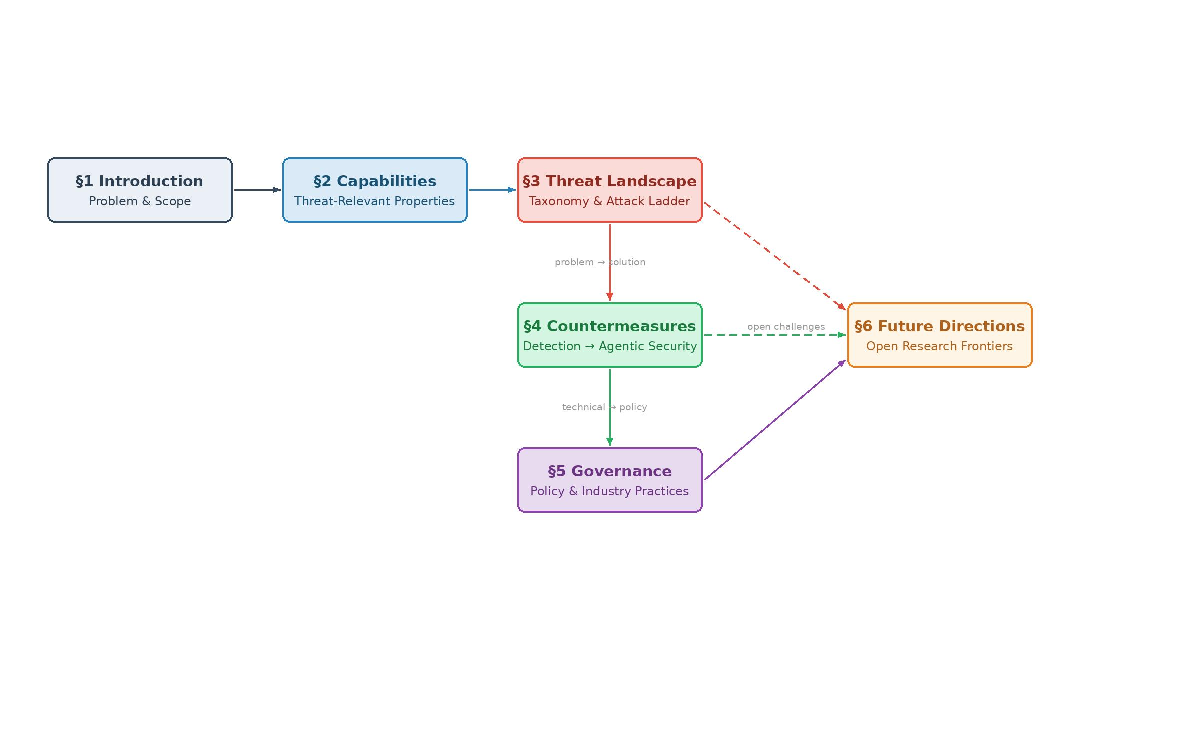
\includegraphics[width=0.95\linewidth]{figure/fig1_paper_structure.pdf}
\caption{Paper structure and logical dependencies. Solid arrows indicate the primary narrative flow; dashed arrows indicate cross-cutting connections to future research directions.}
\label{fig:structure}
\end{figure}
